%------------------------------------------------------------------------------
%Description       : DDMoRe WP7.2.1 Functional Specification for the Model
%                                   Repository Infrastructure - Introduction 
%Authors           : Mihai Glonț <mglont@ebi.ac.uk>
%                    Camille Laibe <laibe@ebi.ac.uk>
%Organization      : EMBL-EBI
%                    Wellcome Trust Genome Campus
%                    Hinxton
%                    Cambridge
%                    United Kingdom
%------------------------------------------------------------------------------
\section{Introduction}
\label{introduction}
This document provides a detailed description of the functionality that will be provided by the \ddmore Model Repository. The guidelines herein apply not only to the public Repository, but also to any private instances of it.

\subsection{Scope}
This document reviews the characteristics of the \ddmore Model Repository in relation to the wider context of the project, outlining along the way envisaged workflows, interactions with both users and third party software, as well as potential software dependencies of the Repository. The intended audience for this specification are the EFPIA and academic partners that wish to use the Repository in an optimal manner, or are merely interested in its capabilities.

\subsection{Non-Goals}
Although this task should deliver a technical specification at this stage according to the Description of Work, it is paramount that the behaviour of the Repository meets the needs of its end-users. Therefore, this document aims to offer a mental picture of the features that have been incorporated into the design of the Repository, allowing the interested stakeholders to flag up any shortcomings. Implementation-specific details about the inner-workings of the Repository are outside of the scope of this document, but will be discussed in the second technical specification which is due in month 42 of the project. 

\subsection{Context}
\label{context}
In a world where inefficient data and knowledge-sharing between academia, pharmaceutical companies and regulatory bodies hinders the development of better medicines, the Drug Disease Model Resources project (\ddmore) -- a Europe-wide effort funded by Innovative Medicines Initiative Joint Undertaking -- seeks to create an environment governed by standards that addresses these shortcomings. Specifically, the \ddmore consortium is developing a common definition language for data, models and work flows, as well as a standard for storing and exchanging \glspl{model} and associated \gls{metadata}\cite{ddmore:dow}.

The main focus on this specification is the objective of Task 7.2: the \ddmore Model Repository. It aims to provide a central repository for the models created by the project, encouraging their reuse. The Repository is closely linked with other deliverables of \ddmore. For instance, the pre-competitive models that will populate the Model Repository initially will be provided by Work Package 1. The models will be encoded in the XML-based format developed by WP4, and the Repository will rely on the software library created by Task 2.3 in order to manipulate the models. Finally, the published models stored in the \ddmore Model Repository will be showcased in the public instance of the Modelling Framework, generated by Task 7.1.

\subsection{Objectives}
\label{objectives}
The main objectives of the Repository are to provide:
\begin{itemize}
  \item a central, versioned, storage place for public and private models
  \item a way to display individual models
  \item a way to search for models
  \item a way to download models
  \item various means to access the stored \glspl{model}, making available the information encoded in MML to both users and tools. 
\end{itemize}

\subsection{Type of users}
\label{users}
This section classifies the users of the \ddmore Model Repository into categories. With the exception of Administrators, whose permissions are granted at global level, over the entire instance of the Repository, all other roles that require authentication are defined at the level of a specific revision. This means that the owner of one model can also be the editor of a revision for another model. 

\begin{description}
  \item[Visitor] an anonymous user accessing \glspl{published model}.
  \item[Owner] the user who submitted the model and has ultimate ownership of what is done to it and how and
when it is published.
  \item[Editor] any user who is able to modify and add information to an existing published or \gls{unpublished model}. Typically the Owner of a model is also an Editor of this model.
  \item[Collaborator] any user who is able to access an unpublished model.
  \item[Reviewer] a user who can access an unpublished model. This role can be limited in time.
  \item[Administrator] a user who is responsible for the security, management and maintenance of the system.
\end{description}

The interactions between users, the Model Repository and other components of the project (such as the Interoperability Framework) are depicted in Figure~\ref{fig:userInteraction}. As such, one may access the Repository directly -- through the web-based user interface -- or indirectly, via the Modelling Interoperability Framework, that uses the Task Execution Language (TEL) and the software library created in WP2.3 to access and store models in the \ddmore Model Repository.

\begin{figure}[htb]
\centering
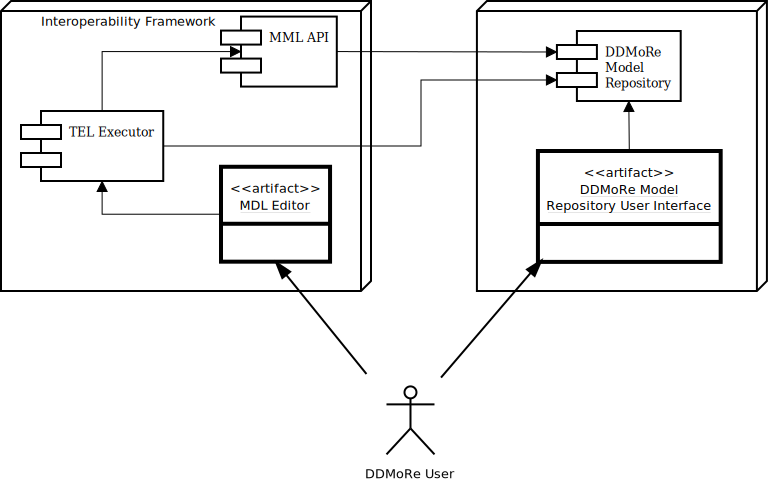
\includegraphics{img/UserInteraction}
\caption{Interactions between users, the interoperability framework and the Model Repository.}
\label{fig:userInteraction}
\end{figure}
